\documentclass[preprint]{aastex}
\usepackage{amsmath, amsfonts, amssymb}
\usepackage{fullpage}
\usepackage[colorlinks,urlcolor=blue,citecolor=blue,linkcolor=blue]{hyperref}

\slugcomment{Draft: \today}
\shorttitle{ATA Beam Squint}
\shortauthors{Burns et al.}

\begin{document}
\title{Characterizing Beam Size and Squint at the ATA}
\author{Keaton J. Burns, Peter K. G. Williams, \and Geoffrey C. Bower}

\begin{abstract}
We present a study of primary beam size and squint in the antennas and
feeds at the Allen Telescope Array, based on weekly calibrator
observations in small mosaicked patterns. A relational database of
beam parameters was created, which reduces the results of an upgraded
and automated analysis pipeline.  A Python visualization tool was
developed to efficiently interface with the squint database and search
for correlations in this large dataset.  We find that \ldots
\end{abstract}


%%%%%
\section{Introduction}\label{s.intro}
ATA telescope calibration is accomplished through observing known
radio point sources to determine the system temperature, pointing
centers, and beam shape for each antenna.  One parameter of interest
from these observations is telescope squint, which we define as the
offset of the Y polarization pointing center from the X polarization
pointing center, in azimuth and altitude.  Knowledge of each
telescope's squint is useful for assessing the reliability of data
from each polarization based on each telescope's pointing model
(e.g., for large-squint telescopes, pointing models based on X
polarization pointing centers yield suboptimal Y polarization
data). Studying telescope squint also provides insights into the
strengths and limitations of the offset-Gregorian dish and
log-periodic feed designs used at the ATA, and may be useful for
directing future telescope development.  Our aims in this project
included isolating the cause of the squint to the feed or dish,
studying the effects of feed upgrades on the squint, and assessing the
stability of a telescope's squint with changes in frequency and time.


%%%%%
\section{Data Collection}\label{s.datacollection}

\subsection{Observations}\label{ss.observations}
The \text{hex} observing routine consists of a central pointing at a known
radio point source and six pointings in a hexagonal pattern around the
source, and are generally completed once each week.  Flux measurements
are recorded for each antenna and polarization (antpol). Observations
have most often been taken using two correlators at 700 \& 1430, 2009
\& 3140, and 5000 \& 7600 MHz, with the focus set for the higher of
each pair of frequencies, and the hexagonal observations at the
nominal primary beam FWHM for that frequency.  Each of these three
observations takes roughly 18 minutes. We expect data at 1430 and 3140
MHz to be the most accurate, since these observations are the most
numerous and were in focus. The radio sources 3c48, 3c138, 3c147, and
3c286 were used as targets.

\subsection{Data Reduction}\label{ss.reduction}
Part of the data reduction includes fitting a two-dimensional Gaussian
function to the relative gains at each of the seven pointings for each
antpol.  This procedure provides a measurement of the actual primary
beam of the telescope at the observed frequency with respect to the
contemporary pointing model.  The center and width uncertainties, the
reduced $\chi^2$ value of the fit and the system equivalent flux
density (SEFD) for each antpol were also calculated.

The reduced beam parameters from all runs were imported into a
relational database for analysis.  A query program use the Structured
Query Language (SQL) to retrieve and plot data with arbitrary
filtering and transformation of the underlying values. Derived data
such as squint magnitudes and angles, and their respective
uncertainties, are computed during retrieval.

\subsection{Outlier Removal}\label{ss.outliers}
A mechanism was implemented to exclude bad data from downstream
analyses.  To remove bad observations, and particularly poor reduction
fits, observations with frequency-normalized squint or width
components in the top percentile, or uncertainties above the
98$^\textrm{th}$ percentile, were flagged as outliers.  Observations
above the 98$^\textrm{th}$ percentile of SEFD and the 90$^\textrm{th}$
percentile of the Gaussian fit $\chi^2$ value were also flagged.  The
$\chi^2$ cutoff is at a significantly lower percentile, as it is a
direct indicator of the convergence of the Gaussian fits, and there
were a significant number of outliers in this parameter, as shown in
Fig.~\ref{fig.dist_sumchisq}.

Nearly all observations at 700 MHz, the lowest observed frequency,
were flagged under these conditions, so the remaining observations
were also excluded.  Additionally, data at 3140 MHz revealed a strong
beam size and shape dependence on the observed source, seemingly
caused by source confusion, prompting us to discard all but the 3c48
observations (see Fig.~\ref{fig.source_confusion}). After removal of
these data, 1309 observations remained.

\begin{figure}[htb]
\begin{center}
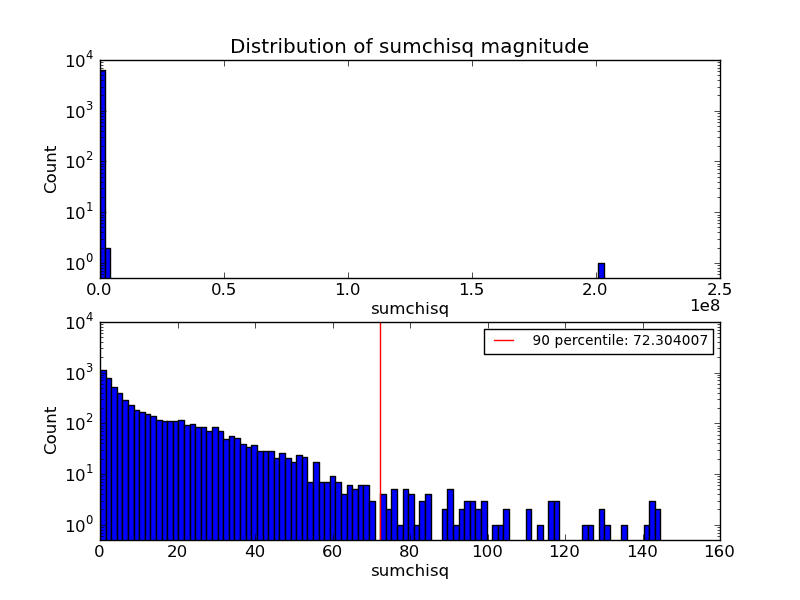
\includegraphics[width=0.7\textwidth]{images/dist_sumchisq}
\caption{Top: Distribution of $\chi^2$ values for 2D Gaussian primary
  beam fits across all observations.  Bottom: Zoom-in at outlier
  cutoff at the 90$\textrm{th}$ percentile. \label{fig.dist_sumchisq}}
\end{center}
\end{figure}

\begin{figure}[htb]
\begin{center}
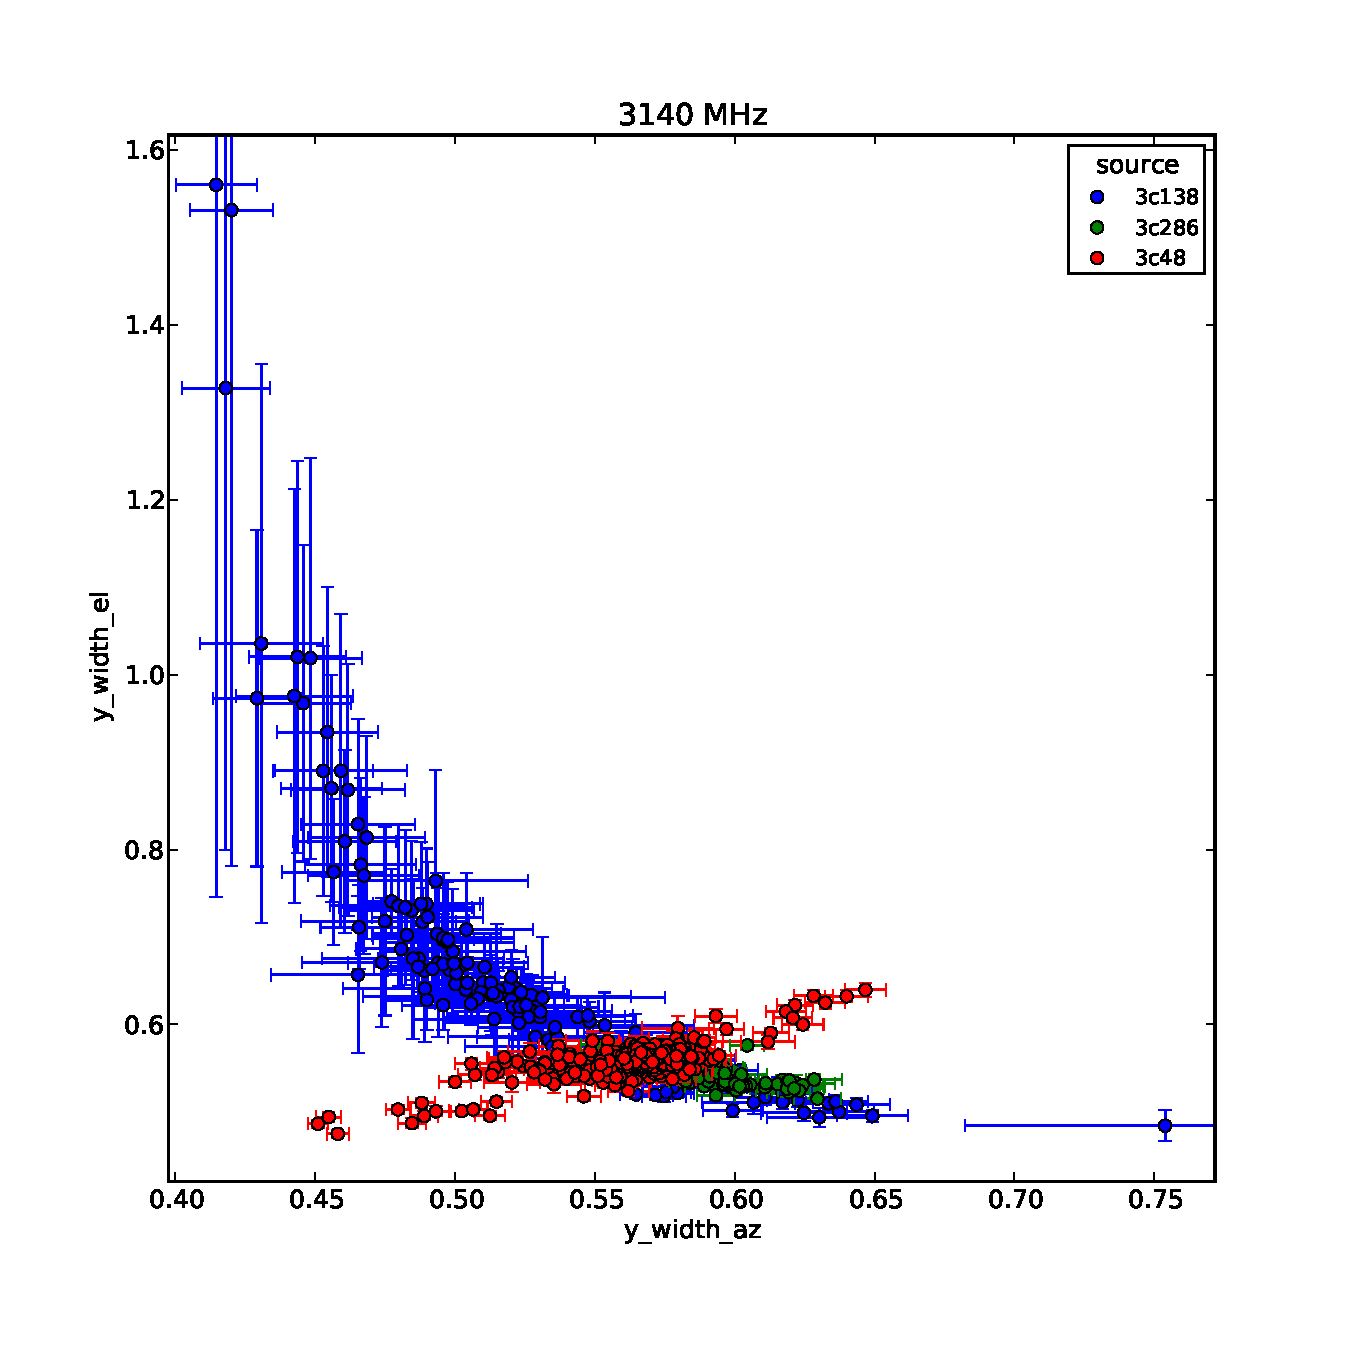
\includegraphics[width=0.8\textwidth]{images/source_confusion}
\caption{Source confusion in 3140 MHz observations.  Source 3c48 used
  for analysis. \label{fig.source_confusion}}
\end{center}
\end{figure}


%%%%%
\section{Analysis and Results}\label{s.results}

\subsection{Primary Beam Size}\label{ss.beamsize}
Scatterplots depicting the primary beam shape (best-fit 2D Gaussian
elevation width vs azimuthal width) for the X and Y polarizations are
depicting in Figures~\ref{fig.x_widths} and \ref{fig.y_widths}
respectively, and Table \ref{tab.widths} gives the means and standard
deviations of these values.  We find general agreement with the
approximate results of \citet{Harp2011}, namely $\textrm{FWHM} \approx
3.5^{\circ} / f_\textrm{GHz}$.

\begin{table}[htb]
\begin{center}
\begin{tabular}{cccc}
Polarization & Direction & Mean [$^{\circ} / f_\textrm{GHz}$] & St. Dev \\
\hline
X & El & 3.663 & 0.245 \\
X & Az & 3.443 & 0.216 \\
Y & El & 3.568 & 0.331 \\
Y & Az & 3.568 & 0.303
\end{tabular}
\caption{Best-fit primary beam width averages \label{tab.widths}}
\end{center}
\end{table}

\begin{figure}[htb]
\begin{center}
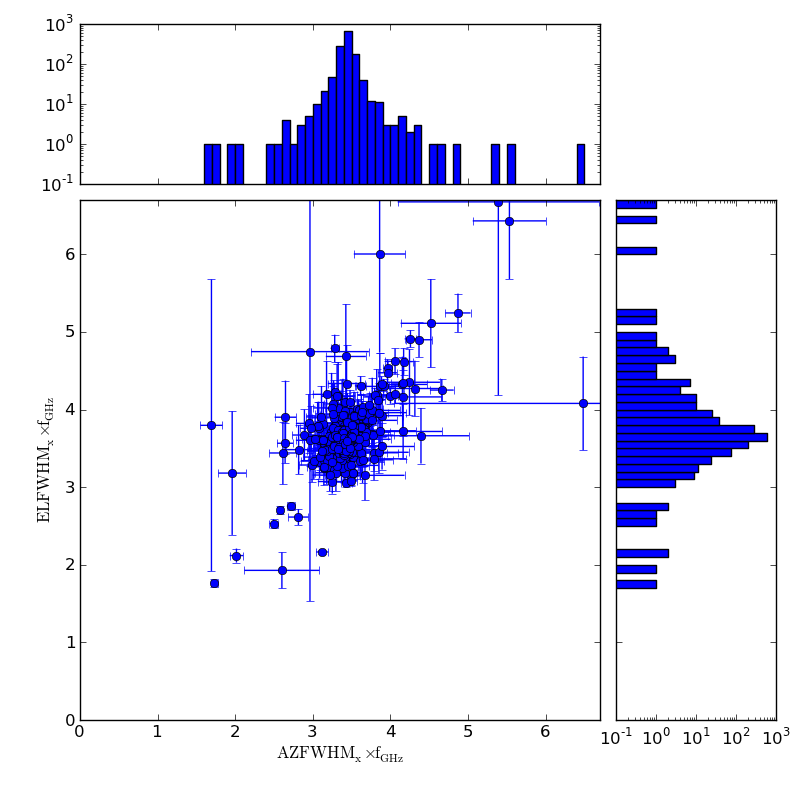
\includegraphics[width=0.8\textwidth]{images/x_widths}
\caption{X polarization primary beam widths. \label{fig.x_widths}}
\end{center}
\end{figure}

\begin{figure}[htb]
\begin{center}
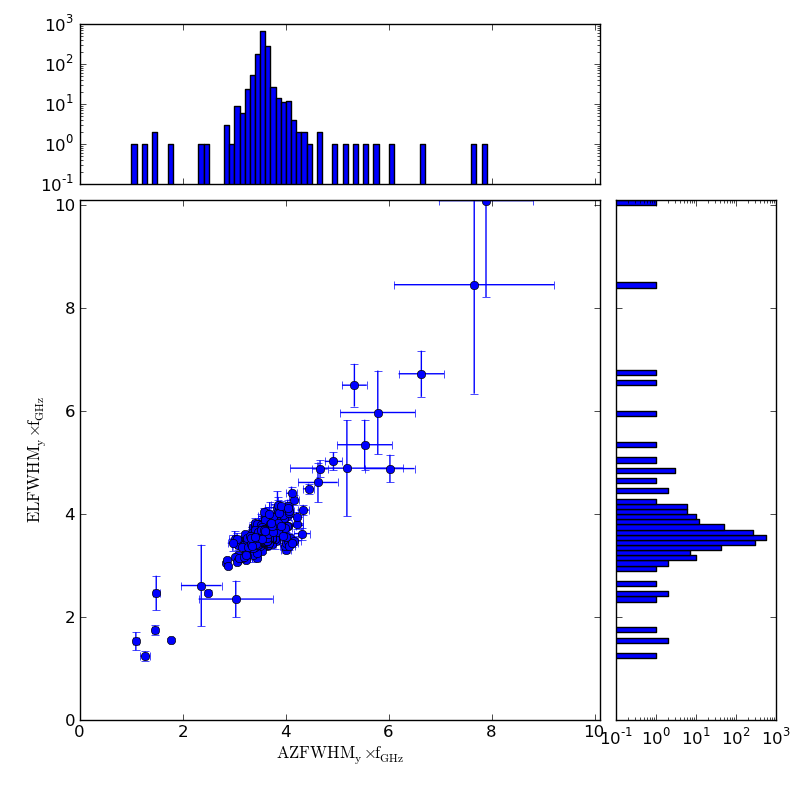
\includegraphics[width=0.8\textwidth]{images/y_widths}
\caption{Y polarization primary beam widths. \label{fig.y_widths}}
\end{center}
\end{figure}

\subsection{Squint: Temporal Variation}\label{ss.temporal}

\subsection{Squint: Feed vs. Antenna}\label{ss.antfeed}

\subsection{Squint: Effects of Feed Revisions}\label{ss.revisions}

\subsection{Squint: Frequency Dependence}\label{ss.freq}
To study the effects of frequency on squint, for each antfeed, we
performed a linear least-squares fit on the log of squint magnitude
and the log of frequency for each observing run.  The slope of this
fit represents the best fitting power-law index $\alpha$, assuming
$|\vec{S}| \propto f^\alpha$.  We then took the median power-law index
across all observing runs for each antfeed.

The best fitting linear slope was similarly computed for each antfeed
(fitting squint magnitude to frequency, assuming a power-law index of
1).  Histograms of these indices and slopes are displayed in figure
NEEDREF.  The same plots were generated with the data separated by
feed revision.  We notice substantial spread in the power-law indices,
mainly between 0 and -2.  We note that the data for for feed revision
3 show less spread (0 to -1) than the other revisions.

%%%%%
\section{Conclusions}\label{s.conclusions}


%%%%%
\bibliographystyle{yahapj}
\bibliography{ATA.bib}

\end{document}
